\lecture{11}{12/2}
We are going to finish off the loose-ends from the proof from
last lecture.
\begin{proof}
    \hfill
    \begin{description}
        \item[$D_0$ is open]
            Given $w \in D_0$, there exists $r>0$ such that $h(z) = 0$
            for all $z \in B_r(w)$. 
            For $z \in B_r(w)$, there exists $r' > 0$ such that
            $B_{r'} \subset B_r(w)$. Hence $h(z') = 0$ for all
            $z' \in B_{r'}(z)$. 
            Hence $z \in D_0$
            therefore $B_r(w) \subset D_0$ hence $D_0$ is open.
            
        \item[$D_1$ is open]
            $D_1 = \bigcup_{n = 0}^\infty (h^{(n)})^{-1}(\C^\star)$.
            $C^\star$ is open and $h^{(n)}$ is continuous, so
            each $(h^{(n)})^{-1}(\C^\star)$ is open and so
            $D_1$ is open.

        \item[$D_0 \cup D_1 = D$] Suppose $w \not\in D_1$, so
            $h^{(n)}(w) = 0$ for all $n \geq 0$. Hence
            the power series of $h$ is $0$.
            Therefore $h(z) = 0$ for all $z \in B_r(w)$
            for some $r > 0$.
            Therefore $w \in D_0$ hence $D_0 \cup D_1 = D$.

        \item[$D_0 \cap D_1 = \varnothing$]
            Suppose $w \in D_0$ then $h \equiv h$ on some
            $B_r(w)$, $r>0$. Therefore
            $h^{(n)}(w) = 0$ for all $n \geq 0$.
            Hence $a \not\in D_1$ and so $D_0 \cap D_1 = \varnothing$.
    \end{description}
\end{proof}

\begin{definition}[]
    Given $S \subset \C$, we say that $w \in S$ is a
    \textbf{non-isolated point} in $S$ if
    for all $\varepsilon > 0$ there exists $z \in S$ such that
    \[
        0 < \abs{z - w} < \varepsilon.
    \]
\end{definition}

\begin{theorem}[Identity]
    Let $D \subset \C$ be a domain and $f,g: D\to \C$ be holomorphic.
    If the set 
    \[
        S = \{z \in D: f(z) = g(z)\}
    \]
    contains a non-isolated point then $f \equiv g$ on $D$.
\end{theorem}

\begin{example}
    Suppose $f: \C \to \C$ is holomorphic and
    \[
        f\left(\frac1n\right) = \sin\left(\frac1n\right)
    \]
    for $n = 1,2,3,\ldots$.
    Note that $\left\{\frac1n: n\in\N\right\}$ does \emph{not}
    contain a non-isolated point.
    $f$ and $\sin$ are continuous, therefore
    \[
        f(0) 
        = \lim_{n\to\infty} f\left(\frac1n\right)
        = \lim_{n\to\infty} \sin\left(\frac1n\right)
        = \sin(0) = 0.
    \]
    Then
    \[
        S 
        = \{ z: f(z) = \sin{z} \}
        \supset \left\{ \frac1n: n \in \N \right\} \cup \{0\}
    \]
    so $0$ is a non-isolated point of $S$. 
    Hence $f = \sin$ on $\C$
    (as $\C$ is a domain, and more importantly, is connected).
\end{example}

\begin{proof}[Proof of the identity theorem]
    Let $w$ be a non-isolated point of $S$.
    Let $h(w) = f(w) - g(w)$ (is holomorphic),
    so $h(w) = 0$ as $w \in S$.
    But for $r > 0$, it holds that $h(z) \neq 0$
    for all $z \in B_r^\star(w)$.
    Therefore, $h \equiv 0$
    on some $B_\varepsilon(w)$ where $\varepsilon > 0$
    by the principle of isolated zeros.
    Therefore, by the uniqueness of analytic continuation
    $h \equiv 0$ on $D$ and so $f \equiv g$ on $D$.
\end{proof}

\chapter{Cauchy's theorem and CIF for simple closed contours}

Recall Cauchy's theorem for starlike domains.
Why do specify our domain as being \emph{starlike}?
In reality, it is because it has no \emph{holes}.
More generally, we don't want $\gamma$ to \emph{wrap around a hole}.

\begin{definition}[Simple]
    A closed curve $\gamma: [a,b] \to \C$ is \textbf{simple}
    if $\gamma(t_1) = \gamma(t_2)$ with $t_1 < t_2$
    implies $t_1 = a$, $t_2 = b$.
\end{definition}

\begin{figure}[]
    \centering
    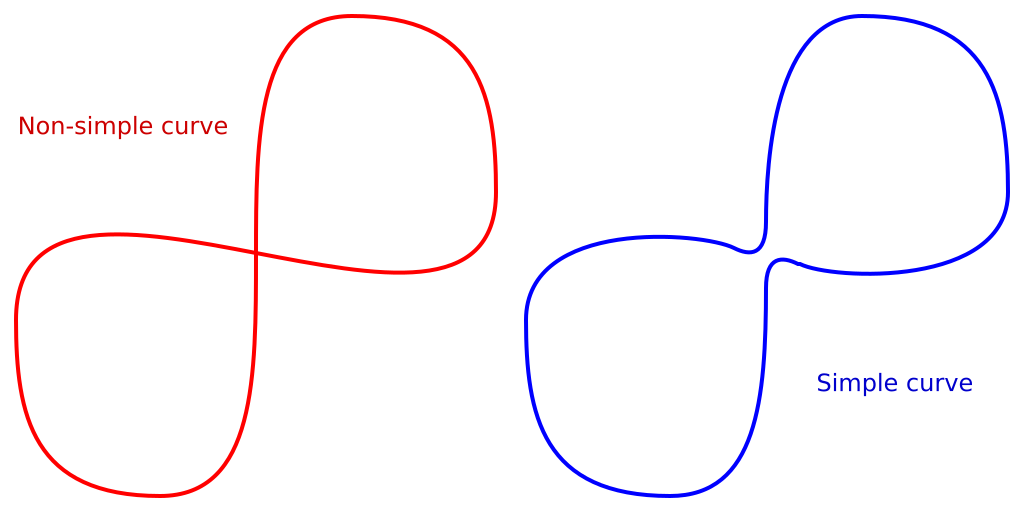
\includegraphics[width=0.8\linewidth]{images/simple-non-simple-closed-curve.png}
    \caption{An example of a simple and a non-simple curve.}
    \label{fig:simple-non-simple-closed-curve}
\end{figure}

\begin{theorem}[Jordan curve]
    Let $\gamma \subset \C$ be a simple closed curve.
    Then its complement $\C \setminus \gamma$ is a disjoint
    union of two domains, exactly one of them is bounded.
\end{theorem}

We will call the bounded domain the \emph{interior} of $\gamma$,
and we will be denoting it by $D_\gamma^\text{int}$.
The other will be called the \emph{exterior} of $\gamma$, denoting it
$D_\gamma^\text{ext}$. For a point $w \in \C \setminus \gamma$,
we will say that $w$ lies inside $\gamma$ if $w \in D^\text{int}_\gamma$
and outside if $w \in D_\gamma^\text{ext}$.

Given a simple closed \emph{contour} $\gamma$, it is possible to pick a
orientation of $\gamma$ as we follow $\gamma$, $D^\text{int}_\gamma$
is on the \emph{left} of $\gamma$ as we follow it.
In this case, we say that $\gamma$ is \emph{positively oriented}.
This is equivalent to traversing the curve anticlockwise.
